\chapter{ボルツマン重み、分配関数、理想気体}

\lectureoverview{正規化と平均エネルギーを固定したもとでエントロピーを最大化することにより、平衡確率分布を導出する。次に分配関数から、微分によって平均エネルギー、エントロピー、温度が得られる。理想気体が最初の完全な例を与え、続いて重力への拡張とエネルギー揺らぎの予告が示される。}

\section{制約付きエントロピー問題}

同じ部分系の同一の、非常に弱く相互作用する\(\mathcal N\)個の複製からなる大きな集団から始める。\(n_i\)個の複製が\(i\)番目の状態を占めるならば、
\begin{equation}
 p_i=\frac{n_i}{\mathcal N},
 \qquad
 \sum_i p_i=1.
 \label{eq:sm4-occupation-probability}
\end{equation}
前回の講義で行った多項係数の数え上げにより、複製あたりのエントロピーは
\begin{equation}
 S[p]=-\sum_i p_i\log p_i.
 \label{eq:sm4-entropy}
\end{equation}
となる。これをすべての変数\(p_1,p_2,\ldots\)の通常の関数とみなすことは有用である。その単純な加法的形が計算を可能にするのである。

複製の集まりは固定された全エネルギー\(\mathcal N E\)をもつ。ここで\(E\)は複製あたりの平均エネルギーである。したがって第二の制約は
\begin{equation}
 \sum_i p_iE_i=E.
 \label{eq:sm4-energy-constraint}
\end{equation}
準位\(E_i\)は部分系に属し、右辺の数\(E\)はそれらの確率重み付き平均である。\eqref{eq:sm4-occupation-probability}および\eqref{eq:sm4-energy-constraint}のもとで\eqref{eq:sm4-entropy}を最大化することにより、圧倒的に最も確からしい占有確率が選び出される。

便宜上、\(-S=\sum_i p_i\log p_i\)を最小化する。各制約に対してラグランジュ乗数を一つ導入する：
\begin{equation}
 \begin{aligned}
 \Phi[p;\alpha,\beta]
 &=\sum_i p_i\log p_i\\
 &\quad+\alpha\left(\sum_i p_i-1\right)\\
 &\quad+\beta\left(\sum_i p_iE_i-E\right).
 \end{aligned}
 \label{eq:sm4-augmented-functional}
\end{equation}
\(\alpha\)および\(\beta\)という名称は、まだ物理的な仮定ではない。この段階では、二つの制約を課すために必要な二つの数にすぎない。

\begin{classroomqa}
\audiencequestion{拡張された関数は\(\alpha\)および\(\beta\)の関数でもあるのか。}
\lecturerresponse{はい。\(\alpha\)および\(\beta\)に関して変分すれば、二つの制約が回復される。しかし当面の計算では、これらの乗数を固定して確率\(p_i\)を変分する。それらの値は後で正規化と指定された平均エネルギーによって固定される。\lecturetimestamp{00:09:32--00:09:49}}
\end{classroomqa}

\begin{figure}[t]
\centering
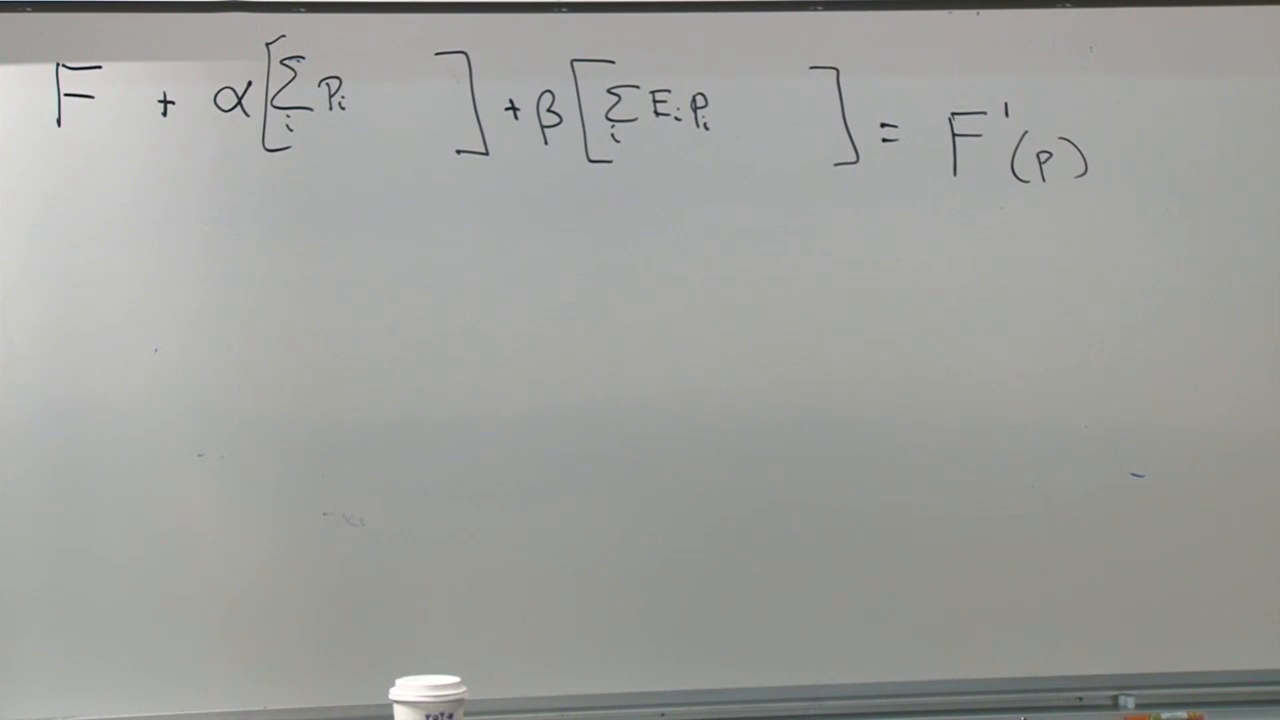
\includegraphics[width=0.92\textwidth]{lecture_04_figure_02.png}
\caption{確率の変分のもとで定数となる項を省略した後の拡張エントロピー汎関数。}
\lectureframe{00:10:56}
\end{figure}

確率に関して微分するとき、項\(-\alpha\)および\(-\beta E\)は何も寄与しない。これが黒板に見える省略された汎関数である。それらは\eqref{eq:sm4-augmented-functional}の一部であり続けるが、この特定の微分には無関係になっただけである。

\section{ボルツマン分布}

任意の一つの確率を選ぶ。講義では\(p_7\)を選ぶ。その理由の一部は、\(1\)が特別すぎるように見えることと、\(7\)が縁起の良い数であることである。この選択に依存するものは何もない。必要な微積分は
\begin{equation}
 \frac{d}{dp_i}\bigl(p_i\log p_i\bigr)=\log p_i+1.
\end{equation}
だけである。したがって
\begin{equation}
 \frac{\partial\Phi}{\partial p_i}
 =\log p_i+1+\alpha+\beta E_i=0.
 \label{eq:sm4-stationarity}
\end{equation}
\(p_i\)について解くと、
\begin{align}
 \log p_i&=-(1+\alpha)-\beta E_i,\\
 p_i&=e^{-(1+\alpha)}e^{-\beta E_i}.
\end{align}
第一の因子は状態ラベルに依存しない。これを\(1/Z\)と書く：
\begin{equation}
 p_i=\frac{e^{-\beta E_i}}{Z}.
 \label{eq:sm4-boltzmann-weight}
\end{equation}

これが最初の突然の報酬である。ありふれた制約付き微分から指数法則が生じた。相対確率は
\begin{equation}
 \frac{p_i}{p_j}=e^{-\beta(E_i-E_j)}.
 \label{eq:sm4-relative-weight}
\end{equation}
に従う。乗数\(\beta\)は、確率がエネルギーとともにどれほど急速に減少するかを制御する。大きな正の\(\beta\)は分布を最低準位の近くに集中させ、小さな正の\(\beta\)はかなりの重みをスペクトルのより上へ広げる。\(\beta\)を変えると平均エネルギーが変わることはすでに見て取れるが、それを逆温度と同定することはまだ証明されなければならない。

\section{正規化と分配関数}

正規化により状態に依存しない因子が決まる：
\begin{equation}
 1=\sum_i p_i
 =\frac{1}{Z}\sum_i e^{-\beta E_i},
\end{equation}
したがって
\begin{equation}
 Z(\beta)=\sum_i e^{-\beta E_i}.
 \label{eq:sm4-partition-function}
\end{equation}
これが正準分配関数である。最初は正規化定数として現れたが、その記述はその役割をひどく過小評価している。\(Z(\beta)\)がわかれば、熱力学的量はその微分から従う。

\eqref{eq:sm4-partition-function}におけるエネルギー準位は入力である。それらは系の力学と、固定された外部条件、すなわち箱の体積と形状、磁場または電場、その他の制御パラメータから来る。制御パラメータを変えるとスペクトルが変わり、したがって\(Z\)が変わる。当面の計算では、それらのパラメータ、ひいては集合\(\{E_i\}\)は固定されている。

\begin{classroomqa}
\audiencequestion{指数関数のスケッチの軸は正確には何を表すのか。縦座標は特定の\(p_i\)の一つなのか。}
\lecturerresponse{プロットされた高さは準位に割り当てられた確率であり、横方向の順序は状態ラベル\(i\)として、あるいはより物理的にはエネルギー\(E_i\)として読むことができる。各状態は固定されたエネルギーをもつ。\(\beta\)が大きいと、確率はそのエネルギーとともに急激に減少する。\(\beta=0\)の近くでは、重みはアクセス可能な準位にわたってほぼ平坦である。
\lecturetimestamp{00:19:39--00:20:09}}
\end{classroomqa}

\section{分配関数に隠れた平均エネルギー}

第二の拘束条件が\(\beta\)を決定する：
\begin{equation}
 E=\sum_i p_iE_i
 =\frac{1}{Z}\sum_i E_i e^{-\beta E_i}.
 \label{eq:sm4-mean-energy}
\end{equation}
この重み付き和を新たに評価するのではなく、
\eqref{eq:sm4-partition-function}を微分する：
\begin{equation}
 \frac{dZ}{d\beta}
 =-\sum_i E_i e^{-\beta E_i}.
\end{equation}
\eqref{eq:sm4-mean-energy}と比較すると
\begin{equation}
 E(\beta)
 =-\frac{1}{Z}\frac{dZ}{d\beta}
 =-\frac{d\log Z}{d\beta}.
 \label{eq:sm4-energy-logz}
\end{equation}
対数が自然対数であるのは、その導関数が因子
\(1/Z\)を与えるからである。

\begin{figure}[t]
\centering
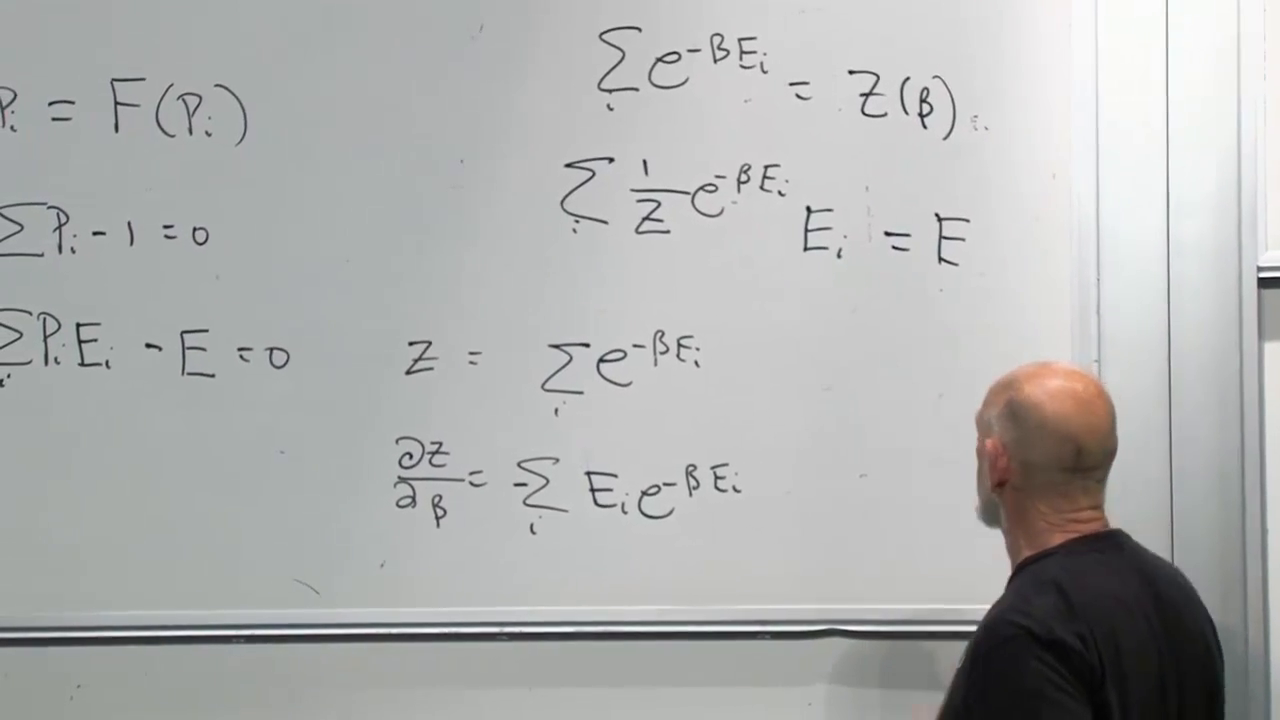
\includegraphics[width=0.82\textwidth]{lecture_04_figure_03.png}
\caption{正規化、平均エネルギーの拘束条件、および分配関数の導関数が黒板上に一緒に現れている。}
\lectureframe{00:26:24}
\end{figure}

\begin{classroomqa}
\audiencequestion{黒板の下の式は\(Z\)に対する新しい式なのか、それともその上の定義から得られるのか。}
\lecturerresponse{それは定義
\(Z=\sum_i e^{-\beta E_i}\)を微分することによって得られる。導関数は
\(-E_i\)を引き下ろす。その結果を\(Z\)で割ると、平均エネルギーを定義する重み付き和が再現される。
\lecturetimestamp{00:25:58--00:26:37}}
\end{classroomqa}

\begin{classroomqa}
\audiencequestion{
\(dZ/d\beta=-E Z\)は\(Z\)を微分の固有関数にするか。}
\lecturerresponse{通常の意味ではそうではない。固有値方程式では\(Z\)に定数が掛かるのに対し、ここでは
\(E=E(\beta)\)である。この式は\(\beta\)の関数としての平均エネルギーを述べているのであり、固定固有値問題ではない。
\lecturetimestamp{00:28:49--00:29:43}}
\end{classroomqa}

\eqref{eq:sm4-energy-logz}の単純さは見かけにすぎない。スペクトルは複雑かもしれず、\(Z\)の計算は困難でありうるが、その一つの関数さえ見つかれば、平均エネルギーは一回の微分で得られる。このパターンは統計力学の至るところで繰り返される：正しい順序で適用された初等的な操作が、直接推測するのは難しかったであろう結果をもたらすのである。

\begin{classroomqa}
\audiencequestion{\(E\)はすべての複製の全エネルギーなのか、それとも一箱あたりの平均エネルギーなのか。}
\lecturerresponse{それは一箱の平均エネルギーである。複製の集まりは全エネルギー\(\mathcal N E\)をもつ。後に、系そのものが\(N\)個の気体粒子を含む一箱全体として選ばれるとき、\(E\)はその気体試料全体のエネルギーを意味することになる。
\lecturetimestamp{00:30:55--00:31:10}}
\end{classroomqa}

\begin{classroomqa}
\audiencequestion{
\(\sum_i e^{-\beta E_i}\)の対数を項ごとに取ることはできるか。}
\lecturerresponse{いいえ。対数は積を和に変えるのであって、和を対数の和に変えるのではない：
\[
 \log\!\left(\sum_i e^{-\beta E_i}\right)
 \ne \sum_i\log\!\left(e^{-\beta E_i}\right).
\]
この区別は、独立な部分系がそれらの分配関数を掛け合わせるようになる後で役に立つ。
\lecturetimestamp{00:31:10--00:31:58}}
\end{classroomqa}

\section{何が固定され、何が変化を許されるのか}

同じ式の中にいくつかの層の変数があり、教室での議論はそれらを意図的に区別している。

\begin{itemize}
 \item 確率\(p_i\)は元々の未知数である。
 \item 準位\(E_i\)は、系とその制御パラメータが指定されれば固定される。
 \item 乗数\(\alpha\)は正規化\(Z=e^{1+\alpha}\)に吸収されている。
 \item 規定された平均エネルギー\(E\)に対して、拘束条件は一つの数\(\beta\)を固定する。しかし平衡状態の族にわたっては、\(E=E(\beta)\)または\(\beta=\beta(E)\)のいずれかを用いることができる。
\end{itemize}

\begin{classroomqa}
\audiencequestion{乗数が数であるなら、なぜ\(\beta\)と\(E\)が今変数として扱われるのか。}
\lecturerresponse{一つの拘束問題に対しては、それらは確かに数である。しかし、同じスペクトルと同じでない規定された平均エネルギーをもつ多くの平衡問題を比較することができる。その族に沿って、\(\beta\)は\(E\)とともに変化する。\(E\)を固定すれば\(\beta\)が決まり、\(\beta\)を固定すれば\(E\)が決まる。これらは同じ関係の二つの読み方である。
\lecturetimestamp{00:31:58--00:33:27}}
\end{classroomqa}

\begin{classroomqa}
\audiencequestion{\(\alpha\)は消えてしまったのか。}
\lecturerresponse{消えたのはその名前だけである。定義
\(e^{-(1+\alpha)}=1/Z\)がそれを\(Z\)に吸収する。\(\alpha\)と\(Z\)の両方を保つと、同じ正規化パラメータを二重に数えることになる。
\lecturetimestamp{00:33:29--00:33:49}}
\end{classroomqa}

エネルギーだけが唯一の保存量である必要はない。全運動量、粒子数、角運動量、または別の量が拘束されているなら、その期待値はそれ自身の乗数を受け取る。その拡張はアンサンブルを変えるが、方法は変えない。

\begin{classroomqa}
\audiencequestion{平均エネルギーだけを固定することは、系についてあまりに多くを仮定しすぎるのではないか。}
\lecturerresponse{それは、現在の問題において条件付けを必要とする他の保存量が存在しないことを仮定している。たとえば全運動量も固定されているなら、別の拘束条件と別のラグランジュ乗数を加えればよい。対照的に、体積、形状、および外部場はここでは制御パラメータである：それらは固定されており、エネルギー準位そのものを決定する。
\lecturetimestamp{00:33:51--00:35:50}}
\end{classroomqa}

\begin{classroomqa}
\audiencequestion{\(\alpha\) はエネルギーのもう一つの引数として現れるべきなのか、また \(Z\) は準位 \(E_i\) に依存するのか。}
\lecturerresponse{\(\alpha\) はすでに \(Z\) に含まれているので、独立な引数ではない。分配関数は確かに固定されたスペクトルにも \(\beta\) にも依存する。制御パラメータを変えると \(E_i\) が変わり、したがって \(Z\) も変わる。現在の \(\beta\) に関する微分の間は、スペクトルは固定して保たれる。
\lecturetimestamp{00:35:52--00:37:10}}
\end{classroomqa}

\begin{classroomqa}
\audiencequestion{我々は個々の準位\(E_i\)を変化させているのか、それとも平均エネルギー\(E\)を変化させているのか。}
\lecturerresponse{個々の準位は固定されたままである。平均エネルギーは確率が変化するために変化する。したがって、この族は\(E\)によって、あるいは同等に\(\beta\)によってパラメータ付けられ、同じ準位のリスト\(\{E_i\}\)が全体を通して用いられる。
\lecturetimestamp{00:37:12--00:39:04}}
\end{classroomqa}

実際には、温度は気体の全エネルギーよりもはるかに測定しやすいことが多い。温度計を挿入することができる。相対論的質量差を秤量して\(E=mc^2\)を援用するのは正しいが、著しく役に立たない。\(\beta\)を操作可能にするには、今度はそれを温度の熱力学的定義に結び付けなければならない。

\section{温度より先にエントロピー}

エントロピーが論理的には先に来る。ボルツマン確率を\eqref{eq:sm4-entropy}に代入すると、
\begin{equation}
 \log p_i=-\beta E_i-\log Z.
\end{equation}
すると
\begin{align}
 S
 &=-\sum_i p_i\log p_i\\
 &=\beta\sum_i p_iE_i+\log Z\sum_i p_i\\
 &=\beta E+\log Z.
 \label{eq:sm4-entropy-logz}
\end{align}
規格化の和が最後の因子1を与える。これはまたヘルムホルツ自由エネルギーの最初の兆候でもある。なぜなら後に\(F_{\mathrm H}=-T\log Z\)となるからである。ただし\(k_B=1\)の単位である。

\begin{classroomqa}
\audiencequestion{第一項の因子\(1/Z\)はどうなったのか。}
\lecturerresponse{それはすでに\(p_i\)の一部である。和\(\sum_i p_iE_i\)は完全な規格化された確率を含み、定義により平均エネルギー\(E\)である。
\lecturetimestamp{00:43:19--00:43:26}}
\end{classroomqa}

\begin{classroomqa}
\audiencequestion{\(S=\beta E+\log Z\)に負号があるべきではないか。}
\lecturerresponse{いいえ。エントロピーは負号で始まるが、\(\log p_i=-\beta E_i-\log Z\)はさらに二つの負号を含む。それらは\eqref{eq:sm4-entropy-logz}に示された二つの正の項を生じる。
\lecturetimestamp{00:45:53--00:46:03}}
\end{classroomqa}

温度は熱力学的に
\begin{equation}
 dE=T\,dS,
 \qquad
 \frac{1}{T}=\frac{dS}{dE},
 \label{eq:sm4-temperature-definition}
\end{equation}
によって定義された。ただし他のすべての制御パラメータは固定されている。\eqref{eq:sm4-entropy-logz}を直接\(E\)で微分する最初の試みは、\(\beta\)も\(E\)に依存するため、すぐに煩雑になる。全微分を取る方がすっきりしている。
\begin{align}
 dS
 &=\beta\,dE+E\,d\beta
   +\frac{d\log Z}{d\beta}\,d\beta\\
 &=\beta\,dE+E\,d\beta-E\,d\beta\\
 &=\beta\,dE.
 \label{eq:sm4-entropy-differential}
\end{align}
この相殺は\eqref{eq:sm4-energy-logz}を用いている。\eqref{eq:sm4-entropy-differential}と\eqref{eq:sm4-temperature-definition}を比較すると
\begin{equation}
 T=\frac{1}{\beta},
 \qquad
 \beta=\frac{1}{T}.
 \label{eq:sm4-beta-temperature}
\end{equation}

\begin{figure}[t]
\centering
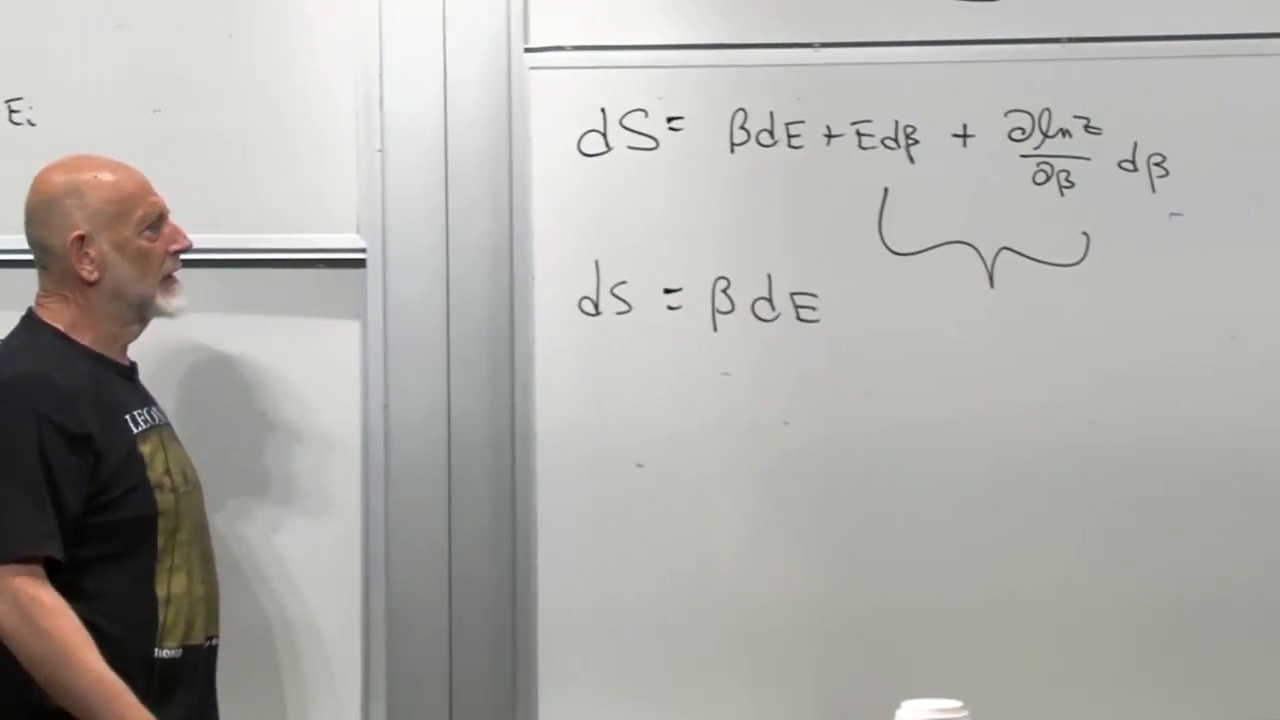
\includegraphics[width=0.82\textwidth]{lecture_04_figure_04.png}
\caption{二つの\(d\beta\)項が相殺し、\(dS=\beta\,dE\)が残る。}
\lectureframe{00:50:48}
\end{figure}

\begin{classroomqa}
\audiencequestion{この相殺は\(\log Z\)がエネルギーや温度から独立であると誤って仮定しているのではないか。}
\lecturerresponse{いいえ。固定されたスペクトルに対しては、独立な熱的パラメータが一つある。\(Z=Z(\beta)\)と書くことができ、次に平衡族に沿って\(\beta=\beta(E)\)とみなすことができる。全微分は完全な\(d\beta\)依存性を保ち、恒等式\(d\log Z/d\beta=-E\)がまさに相殺を成立させている。
\lecturetimestamp{00:52:04--00:52:44}}
\end{classroomqa}

計算のほとんどの間、温度はエネルギー単位で測られるので、\(k_B=1\)である。実験室単位に戻すと、
\begin{equation}
 \beta=\frac{1}{k_B T_{\mathrm K}},
 \label{eq:sm4-beta-laboratory}
\end{equation}
ここで\(T_{\mathrm K}\)はケルビンで表した絶対温度である。\(T_{\mathrm e}=k_BT_{\mathrm K}\)と書いてから\(\beta=1/T_{\mathrm e}\)を用いるのがしばしば便利である。

\begin{classroomqa}
\audiencequestion{気体のある体積について、系は一分子なのか、それとも全体の集まりなのか。}
\lecturerresponse{それは系をどのように定義するかによる。ここでは系は気体の箱全体であり、したがって\(E\)はそのすべての分子のエネルギーである。十分に希薄な理想気体では、粒子が相互作用しないため、一分子も部分系として扱うことができる。以下の因子分解が二つの記述の関係を示すであろう。
\lecturetimestamp{00:53:32--00:54:49}}
\end{classroomqa}

正準集団の恒等式をここでまとめておく。
\begin{align}
 p_i&=\frac{e^{-\beta E_i}}{Z},&
 Z(\beta)&=\sum_i e^{-\beta E_i},\label{eq:sm4-canonical-pair}\\
 E&=-\frac{d\log Z}{d\beta},&
 S&=\beta E+\log Z,&
 T&=\frac{1}{\beta}.
 \label{eq:sm4-canonical-identities}
\end{align}

\section{古典的理想気体}

体積\(V\)の箱の中に質量\(m\)の同一な点粒子\(N\)個を取る。粒子間の相互作用が無視できるとき、気体は理想的である。これは、力が弱いため、あるいは気体が十分に希薄で近接遭遇が稀であるため、良い近似となりうる。

古典的微視的状態はすべての位置と運動量によって指定される。
\begin{equation}
 (\bm q_1,\ldots,\bm q_N;\bm p_1,\ldots,\bm p_N).
\end{equation}
位置座標が\(3N\)個、運動量座標が\(3N\)個あるので、状態は\(6N\)次元の位相空間の一点である。相互作用がなければ、ハミルトニアンは
\begin{equation}
 H(\bm p)=\sum_{a=1}^{N}\frac{\bm p_a^2}{2m}
 =\sum_{\mu=1}^{3N}\frac{p_\mu^2}{2m}.
 \label{eq:sm4-ideal-hamiltonian}
\end{equation}

\begin{classroomqa}
\audiencequestion{粒子は\(3N\)個あり、すべての運動量成分について和をとると状態を二重に数えることになるのか。}
\lecturerresponse{粒子は\(N\)個、運動量成分は\(3N\)個である。\eqref{eq:sm4-ideal-hamiltonian}の和には、各成分に対して二次の項が1つずつ含まれる。すると相空間積分は各独立成分をちょうど1回ずつ積分するので、その積から二重計数は生じない。
\lecturetimestamp{01:02:29--01:04:04}}
\end{classroomqa}

連続的な古典相空間では、状態和は
\begin{equation}
 Z_N
 =\frac{1}{N!\,h^{3N}}
 \int_{V^N}d^{3N}q
 \int_{\mathbb R^{3N}}d^{3N}p\,
 e^{-\beta H(\bm p)}.
 \label{eq:sm4-classical-partition}
\end{equation}
となる。講義では積分に焦点を当て、相空間のセル\(h^{3N}\)を書かずに同じ表式を記す。これを復元すると\(Z_N\)が無次元になり、古典的な状態数え上げの量子的起源が記録される。\(h\)は\(\beta\)に依存しないので、以下で用いるエネルギー微分を変えない。

位置積分は直ちに実行できる。ハミルトニアンは位置に依存せず、各粒子は箱の中のどこにでも存在しうる：
\begin{equation}
 \int_{V^N}d^{3N}q=V^N.
\end{equation}
運動量積分は\(3N\)個の同一な一次元ガウス積分に因子分解される：
\begin{equation}
 Z_N
 =\frac{V^N}{N!\,h^{3N}}
 \left[
  \int_{-\infty}^{\infty}dp\,
  e^{-\beta p^2/(2m)}
 \right]^{3N}.
 \label{eq:sm4-factorized-gas}
\end{equation}

因子\(1/N!\)は、同一粒子の置換によってのみ異なる配置を同定する。固定された\(N\)と\(V\)における平均エネルギーに対しては、\(\log Z_N\)に\(\beta\)に依存しない定数を加えるだけなので、\(-\partial/\partial\beta\)の下で消える。しかしすべての問いにおいて不要というわけではない：\(h^{3N}\)とともに、無次元の分配関数、示量的なエントロピー、そして整合的な化学ポテンシャルにとって不可欠である。

ここで
\begin{equation}
 x=\sqrt{\frac{\beta}{2m}}\,p,
 \qquad
 dp=\sqrt{\frac{2m}{\beta}}\,dx.
\end{equation}
と置く。ガウス積分は
\begin{align}
 \int_{-\infty}^{\infty}dp\,e^{-\beta p^2/(2m)}
 &=
 \sqrt{\frac{2m}{\beta}}
 \int_{-\infty}^{\infty}dx\,e^{-x^2}\\
 &=\sqrt{\frac{2\pi m}{\beta}}.
 \label{eq:sm4-gaussian}
\end{align}
となる。

\begin{figure}[t]
\centering
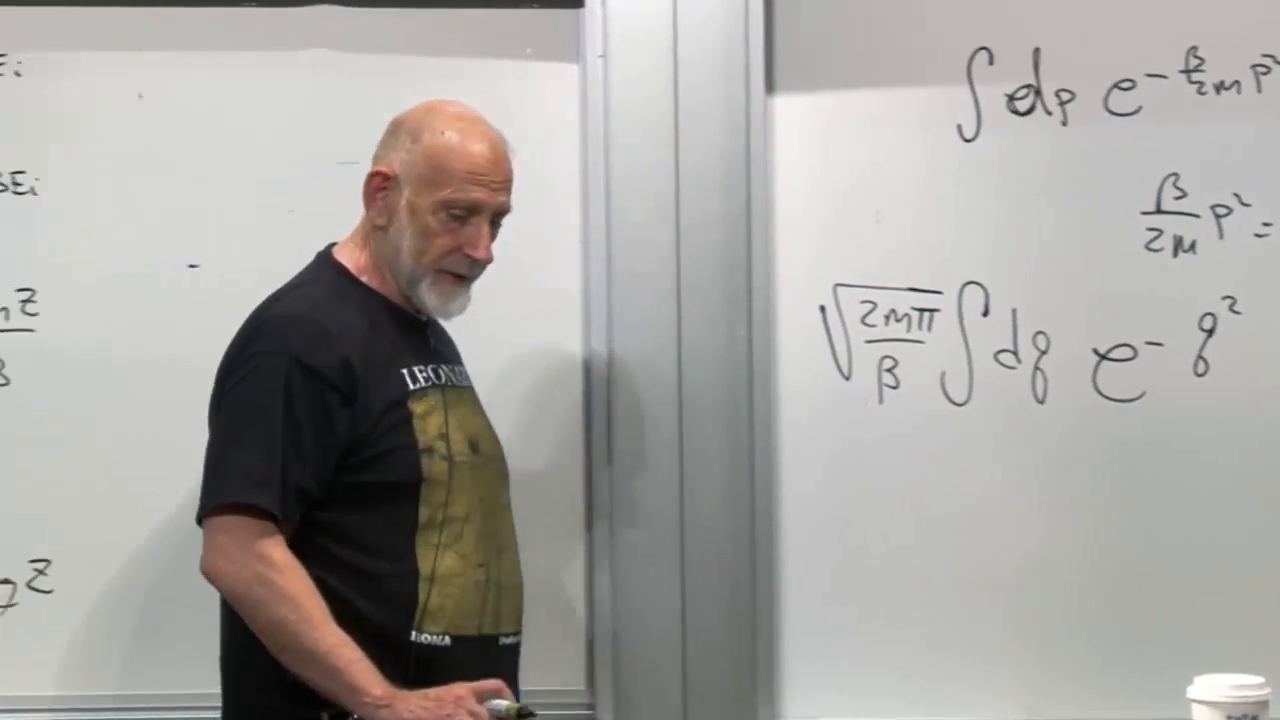
\includegraphics[width=0.82\textwidth]{lecture_04_figure_05.png}
\caption{運動量積分は、1回のスケーリングによって標準的なガウス積分に帰着される。}
\lectureframe{01:13:12}
\end{figure}

\eqref{eq:sm4-factorized-gas}に代入すると
\begin{equation}
 Z_N
 =\frac{V^N}{N!\,h^{3N}}
 \left(\frac{2\pi m}{\beta}\right)^{3N/2}.
 \label{eq:sm4-ideal-partition}
\end{equation}
を得る。

\begin{figure}[t]
\centering
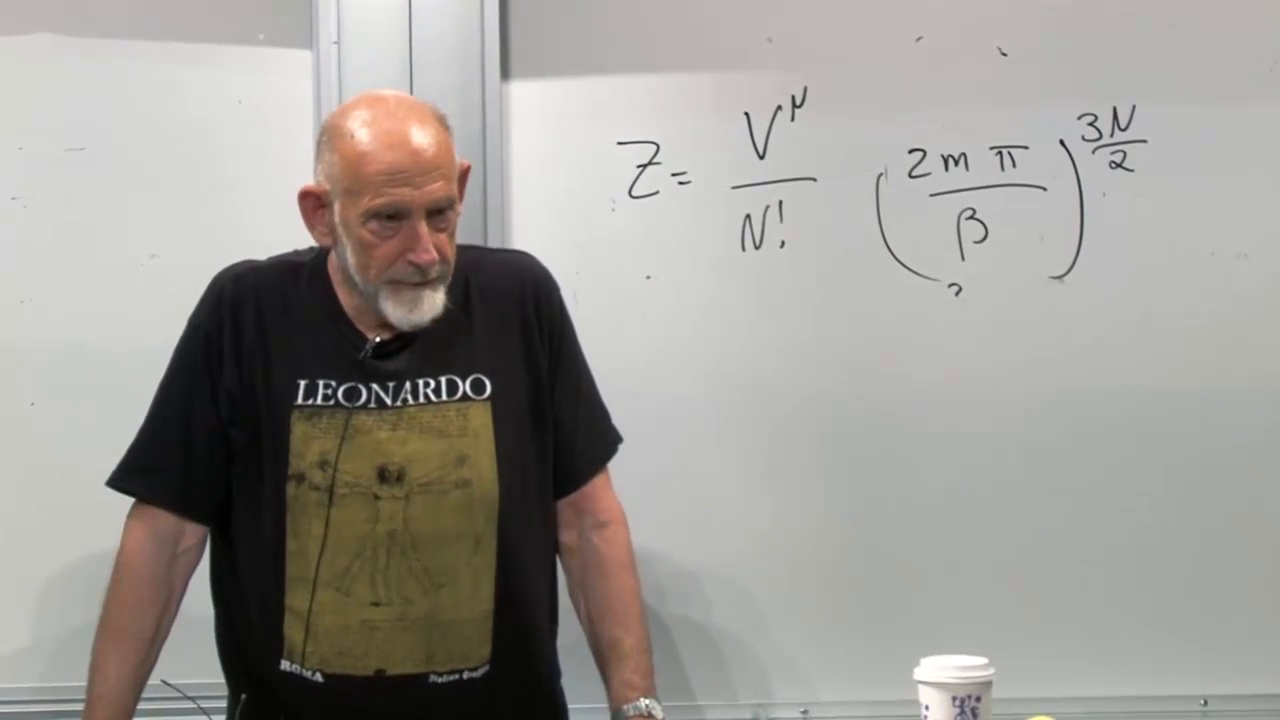
\includegraphics[width=0.78\textwidth]{lecture_04_figure_06.png}
\caption{黒板に完成した理想気体の分配関数。相空間のセル\(h^{3N}\)は\eqref{eq:sm4-ideal-partition}において復元されている。}
\lectureframe{01:14:38}
\end{figure}

同じ結果を熱的ド・ブロイ波長
\begin{equation}
 \lambda_T=\frac{h}{\sqrt{2\pi mT}}
 \qquad (k_B=1).
\end{equation}
でまとめておくと便利である。すると
\begin{equation}
 Z_N=\frac{1}{N!}\left(\frac{V}{\lambda_T^3}\right)^N.
 \label{eq:sm4-thermal-wavelength-form}
\end{equation}
となる。

巨視的な\(N\)に対して、スターリングの公式は
\begin{equation}
 N!\simeq N^Ne^{-N}\sqrt{2\pi N}.
\end{equation}
を与える。主要な指数依存性のみを残し、
\(\rho=N/V\)
と定義すると、
\begin{equation}
 \frac{V^N}{N!}
 \simeq
 \frac{1}{\sqrt{2\pi N}}
 \left(\frac{e}{\rho}\right)^N.
 \label{eq:sm4-density-rewrite}
\end{equation}
となる。これが講義の簡潔な密度による書き換えである。平方根の因子は\(\log Z_N\)において次次の寄与であるが、ここでは黙って落とすのではなく明示している。

\begin{classroomqa}
\audiencequestion{\(1/N!\)が\(\beta\)に依存しないなら、まったく違いを生じないのか。}
\lecturerresponse{固定された\(N\)と\(V\)における現在の平均エネルギー微分には違いを生じない。なぜなら\(\log Z_N\)に\(\beta\)に依存しない定数を加えるからである。しかし絶対エントロピーや粒子数の変動に対しては重要である。限定的な微分についての言明と、より広い状態数え上げについての言明を混同してはならない。
\lecturetimestamp{01:27:01--01:27:51}}
\end{classroomqa}

\section{エネルギーと等分配}

積は微分しにくいが、対数をとれば和になる。\eqref{eq:sm4-ideal-partition}より、
\begin{equation}
 \log Z_N
 =-\frac{3N}{2}\log\beta+\text{\(\beta\)-independent terms}.
 \label{eq:sm4-log-ideal-partition}
\end{equation}
したがって
\begin{equation}
 E
 =-\frac{\partial\log Z_N}{\partial\beta}
 =\frac{3N}{2\beta}
 =\frac{3N}{2}T.
 \label{eq:sm4-ideal-energy}
\end{equation}
粒子あたりのエネルギーは
\begin{equation}
 \frac{E}{N}=\frac{3}{2}T
 \qquad (k_B=1),
\end{equation}
あるいは実験室単位では
\begin{equation}
 \frac{E}{N}=\frac{3}{2}k_BT_{\mathrm K}.
 \label{eq:sm4-ideal-energy-lab}
\end{equation}
である。

\begin{figure}[t]
\centering
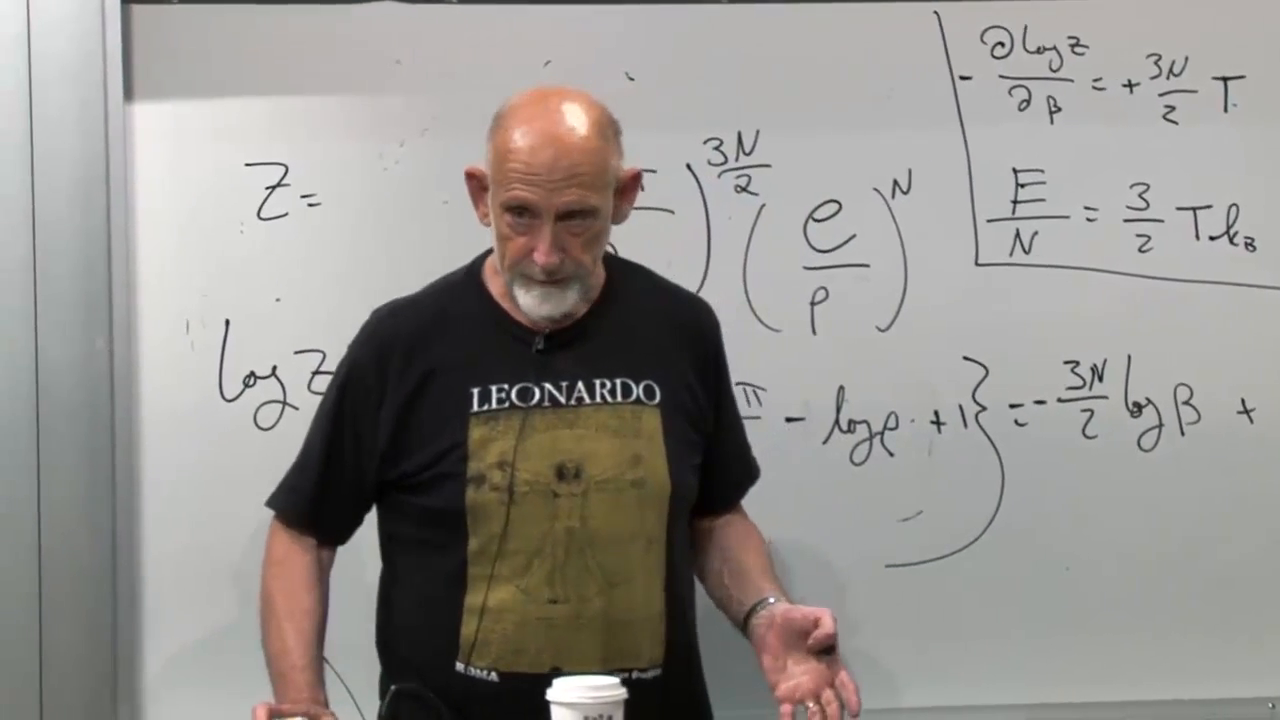
\includegraphics[width=0.84\textwidth]{lecture_04_figure_07.png}
\caption{理想気体のエネルギーに寄与するのは\(-3N\log\beta/2\)の項のみであり、\(E/N=3T/2\)を与える。}
\lectureframe{01:25:28}
\end{figure}

\begin{classroomqa}
\audiencequestion{エネルギーの式にはボルツマン定数はどこから入るのか。}
\lecturerresponse{理論家の温度\(T\)はエネルギーである。ケルビンを用いるには、これを\(k_BT_{\mathrm K}\)に置き換えれば
\(E/N=3k_BT_{\mathrm K}/2\)
となる。\(k_B\)の小さな値が、巨視的に見える数値温度を1分子の微視的エネルギー尺度に変換する。
\lecturetimestamp{01:24:58--01:26:01}}
\end{classroomqa}

3は空間の3方向から来る。1/2は各ガウス積分の\(1/\beta\)への平方根依存性から来る。各独立な二次の運動量座標は平均エネルギーに
\begin{equation}
 \frac{1}{2}T
\end{equation}
を寄与する。\(d\)次元空間では同じ議論により
\(E/N=dT/2\)
となる。これが等分配の最初の出現である。

講義の最後に課題として与えられたエントロピー計算は\(S=\beta E+\log Z_N\)から従う。スターリング近似を用いると、
\begin{equation}
 \frac{S}{N}
 \simeq
 \log\!\left[
  \frac{V}{N}
  \left(\frac{2\pi mT}{h^2}\right)^{3/2}
 \right]
 +\frac{5}{2},
 \label{eq:sm4-sackur-tetrode}
\end{equation}
が、有限\(N\)の次次の補正まで成り立つ。\(k_B\)を復元すると右辺に\(k_B\)が掛かり、\(T\)が\(k_BT_{\mathrm K}\)に置き換わる。この結果は、エネルギーから落ちていた規格化因子がエントロピーにとって不可欠である理由を明らかにする。

\section{気体を重力場に置く}

箱を中性子星の上に置くという問いは、重力への拡張を導入する。中性子星に立ち向かう前に、普通の部屋の中の一様な場\(g\)を考えよう。底面積\(A\)、高さ\(L\)の箱の底面で\(y=0\)を選ぶ。ハミルトニアンは
\begin{equation}
 H=\sum_{a=1}^{N}
 \left(\frac{\bm p_a^2}{2m}+mgy_a\right).
 \label{eq:sm4-gravity-hamiltonian}
\end{equation}
となる。水平方向の位置積分は依然として\(A^N\)を与え、各鉛直座標は
\begin{equation}
 I_y(L)
 =\int_0^Ldy\,e^{-\beta mgy}
 =\frac{1-e^{-\beta mgL}}{\beta mg}.
 \label{eq:sm4-finite-height-integral}
\end{equation}
に寄与する。

\begin{classroomqa}
\audiencequestion{鉛直方向の積分は本当に無限大まで及ぶべきなのか、それとも箱の上端までなのか。}
\lecturerresponse{有限の箱に対しては、\eqref{eq:sm4-finite-height-integral}のように、\(0\)からその高さ\(L\)まで及ばなければならない。上限を無限大にとるのは、有限の部屋ではなく表面上の大気をモデル化する、後段での単純化である。
\lecturetimestamp{01:30:25--01:31:32}}
\end{classroomqa}

したがって、有限の高さに対する完全な分配関数は
\begin{equation}
 Z_N(L)
 =
 \frac{1}{N!\,h^{3N}}
 \left[
  A\,
  \frac{1-e^{-\beta mgL}}{\beta mg}
  \left(\frac{2\pi m}{\beta}\right)^{3/2}
 \right]^N.
 \label{eq:sm4-gravity-partition-finite}
\end{equation}
である。鉛直方向の因子は\(\beta\)に依存するので、エネルギーに寄与しなければならない。実際、
\begin{equation}
 \langle U\rangle
 =N\left[
  \frac{1}{\beta}
  -\frac{mgL}{e^{\beta mgL}-1}
 \right].
 \label{eq:sm4-finite-gravity-energy}
\end{equation}
である。これで、講義で最初は厄介な計算として残された積分の小さな部分が完成する。

無限に高い大気、すなわち\(L\to\infty\)の場合、
\begin{equation}
 I_y(\infty)=\frac{1}{\beta mg}.
\end{equation}
である。分配関数は
\begin{equation}
 Z_N^{(\infty)}
 =
 \frac{1}{N!\,h^{3N}}
 \left[
  \frac{A}{\beta mg}
  \left(\frac{2\pi m}{\beta}\right)^{3/2}
 \right]^N.
 \label{eq:sm4-gravity-partition-infinite}
\end{equation}
となる。その\(\beta\)に依存する対数は
\begin{equation}
 \log Z_N^{(\infty)}
 =-\frac{3N}{2}\log\beta-N\log\beta+\mathrm{const}.
\end{equation}
である。第一項は運動エネルギー\(3NT/2\)を与え、第二項は平均重力ポテンシャルエネルギー\(NT\)を与える。したがって、この理想化された非有界大気に対して
\begin{equation}
 E_{\mathrm{tot}}=\frac{5N}{2}T
\end{equation}
である。

\begin{figure}[t]
\centering
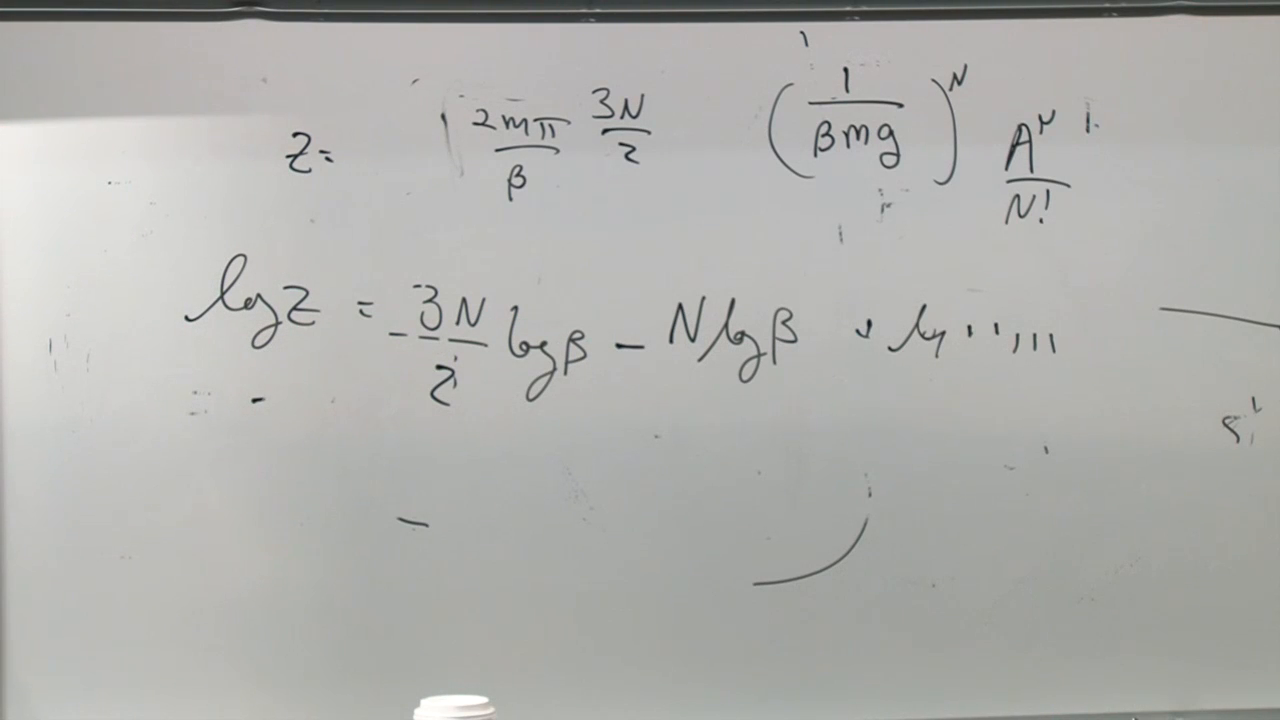
\includegraphics[width=0.83\textwidth]{lecture_04_figure_08.png}
\caption{無限大気の分配関数は、平均ポテンシャルエネルギーの源である\(-N\log\beta\)を\(\log Z\)に加える。}
\lectureframe{01:36:38}
\end{figure}

\begin{classroomqa}
\audiencequestion{非常に強い重力場には別のラグランジュ乗数が必要になるのだろうか。}
\lecturerresponse{単に場が強いからという理由ではない。重力はハミルトニアンを変え、したがってエネルギー準位または位相空間の重みを変える。同じエネルギー乗数\(\beta\)が残る。中性子星はさらなる物理的複雑さをもたらすが、最初の修正は依然として重力ポテンシャルエネルギーを\(H\)に入れることである。
\lecturetimestamp{01:27:58--01:29:24}}
\end{classroomqa}

\section{最後に三つの問い}

\begin{classroomqa}
\audiencequestion{どの方程式がボルツマン分布であり、それは平衡について何を主張するのか。}
\lecturerresponse{その分布は
\[
 p_i=\frac{e^{-\beta E_i}}{Z}.
\]
である。これは規格化と固定された平均エネルギーという条件の下での最大エントロピー分布である。平均エネルギーは同じ確率から計算しなければならず、規格化は最終式ではほとんど自動的に見えても、依然として課さなければならない。
\lecturetimestamp{01:38:14--01:38:45}}
\end{classroomqa}

手順は機械的に感じられるかもしれない。分配関数を書き、対数をとり、微分する。それでも、得られる方程式は驚きに満ち続けている。慣れによって、どの単純な操作がどの操作に続くべきかは分かるが、それによってこの主題の不思議さが減るわけではない。

\begin{classroomqa}
\audiencequestion{これらのエントロピーの考えは、崩壊する恒星やブラックホールに適用できるのか。物質がより小さな領域を占めるのに、どうしてエントロピーが増大しうるのか。}
\lecturerresponse{恒星が難しいのは主に、その物質の詳細が複雑だからである。ブラックホールにはより明快な基準がある。そのベッケンシュタイン--ホーキングエントロピーは、与えられた巨視的制約に対する極限的な重力エントロピーである。崩壊はそのブラックホールの値に達するまでエントロピーを増大させうる。それ以上増大させるには、利用可能なエネルギーまたは大きさを変える必要がある。
\lecturetimestamp{01:39:29--01:40:36}}
\end{classroomqa}

\begin{classroomqa}
\audiencequestion{分配関数はエネルギーの揺らぎも計算できるのか。}
\lecturerresponse{はい。一階微分は平均エネルギーを与え、二階微分はその分散を与える。
\begin{align*}
 \frac{\partial^2\log Z}{\partial\beta^2}
 &=\langle E^2\rangle-\langle E\rangle^2\\
 &=\operatorname{Var}(E).
\end{align*}
エネルギー単位では、これは熱容量と\(\operatorname{Var}(E)=T^2C_V\)の関係にある。実験室単位では、
\(\operatorname{Var}(E)=k_BT_{\mathrm K}^2C_V\)
である。この揺らぎの関係が次の計算である。
\lecturetimestamp{01:40:37--01:41:53}}
\end{classroomqa}

揺らぎは、統計力学を純粋に連続的な熱力学記述から区別する。特にギブズとアインシュタインに結びつけられるその系統的研究は、滑らかな巨視的法則の背後にある有限の微視的構成要素を明らかにする。次回の講義はそこから始まる。